\begin{itemize}
    \item Differential equation~\eqref{eq:odd-exponential-identity} can be expressed in terms of backward
    and central differentials, as well as its dynamic equation analogs~\cite{kolosov2016study}
    \item Definition~\eqref{eq:definition_polynomial_p} is closely related to discrete convolution, probably
    some new identities in term of discrete convolution may be found
    \item All kind of derivatives (forward, backward, central), including time scale ones can be expressed
    as double limit similarly to~\cite{kolosov_2024_10575485}
    \item Equation~\eqref{eq:definition_polynomial_p} approximates odd-power $2m+1$ in some neighborhood of fixed point
    $a$ as it shown on the graphs
    \begin{figure}[H]
        \centering
        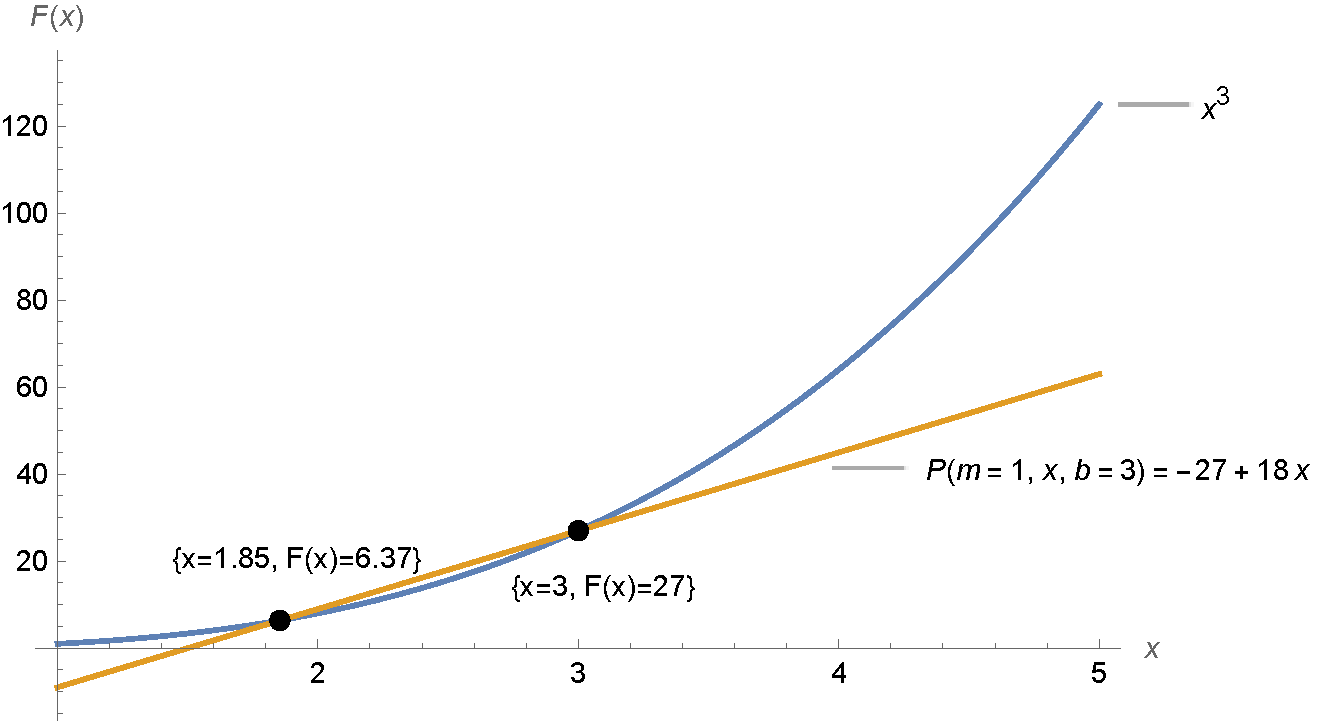
\includegraphics[width=0.6\textwidth]{images/n^3_approximation_m1_b3}
        ~\caption{Approximation of $x^3$.}\label{fig:approximation-n3}
    \end{figure}
    \begin{figure}[H]
        \centering
        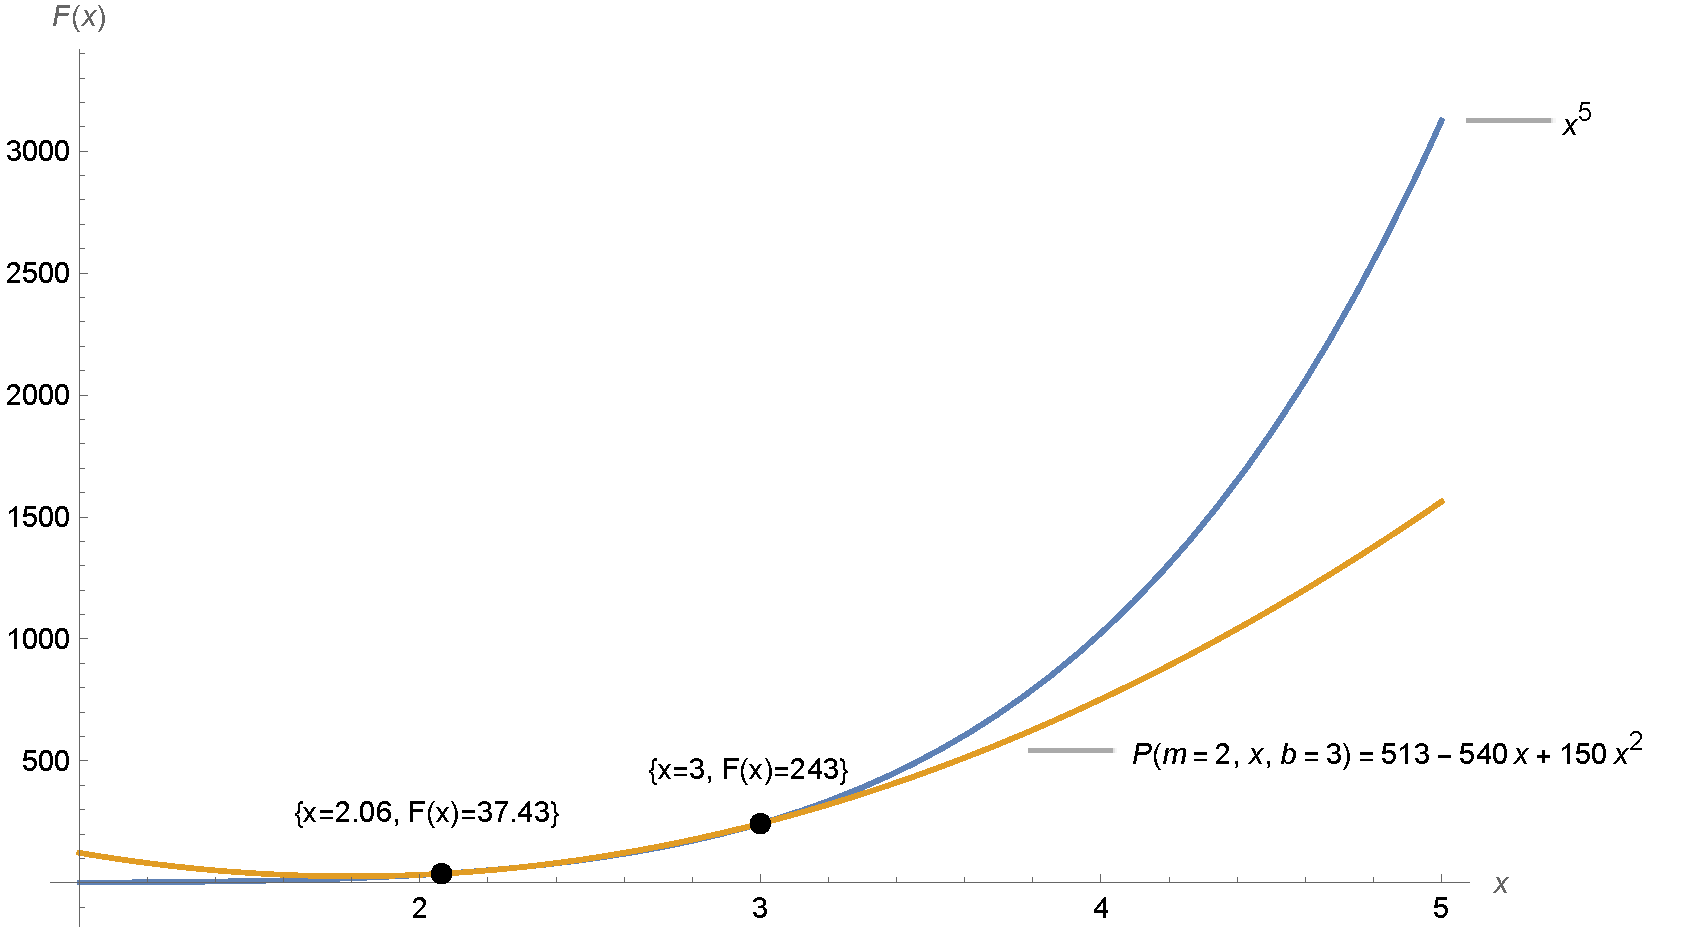
\includegraphics[width=0.6\textwidth]{images/n^5_approximation_m2_b3}
        ~\caption{Approximation of $x^5$.}\label{fig:approximation-n5}
    \end{figure}
    Similar approximations are partially revealed and discussed in \url{https://arxiv.org/pdf/1603.02468v15.pdf}.
    \item Improvements and suggestions to current manuscript via open-source activities at
    \url{https://github.com/kolosovpetro/HistoryAndOverviewOfPolynomialP}
\end{itemize}
